%-----------------------------------------------------------------------------------------------%
%
% Maret 2019
% Template Latex untuk Tugas Akhir Program Studi Sistem informasi ini
% dikembangkan oleh Inggih Permana (inggihjava@gmail.com)
%
% Template ini dikembangkan dari template yang dibuat oleh Andreas Febrian (Fasilkom UI 2003).
%
% Orang yang cerdas adalah orang yang paling banyak mengingat kematian.
%
%-----------------------------------------------------------------------------------------------%

%-----------------------------------------------------------------------------%
%\prefikLampiran{A}

\renewcommand{\thepage}{D - \arabic{page}}
\chapter{\textit{SOURCE CODE}}
%-----------------------------------------------------------------------------%
\begin{figure}[h]
	\centering
	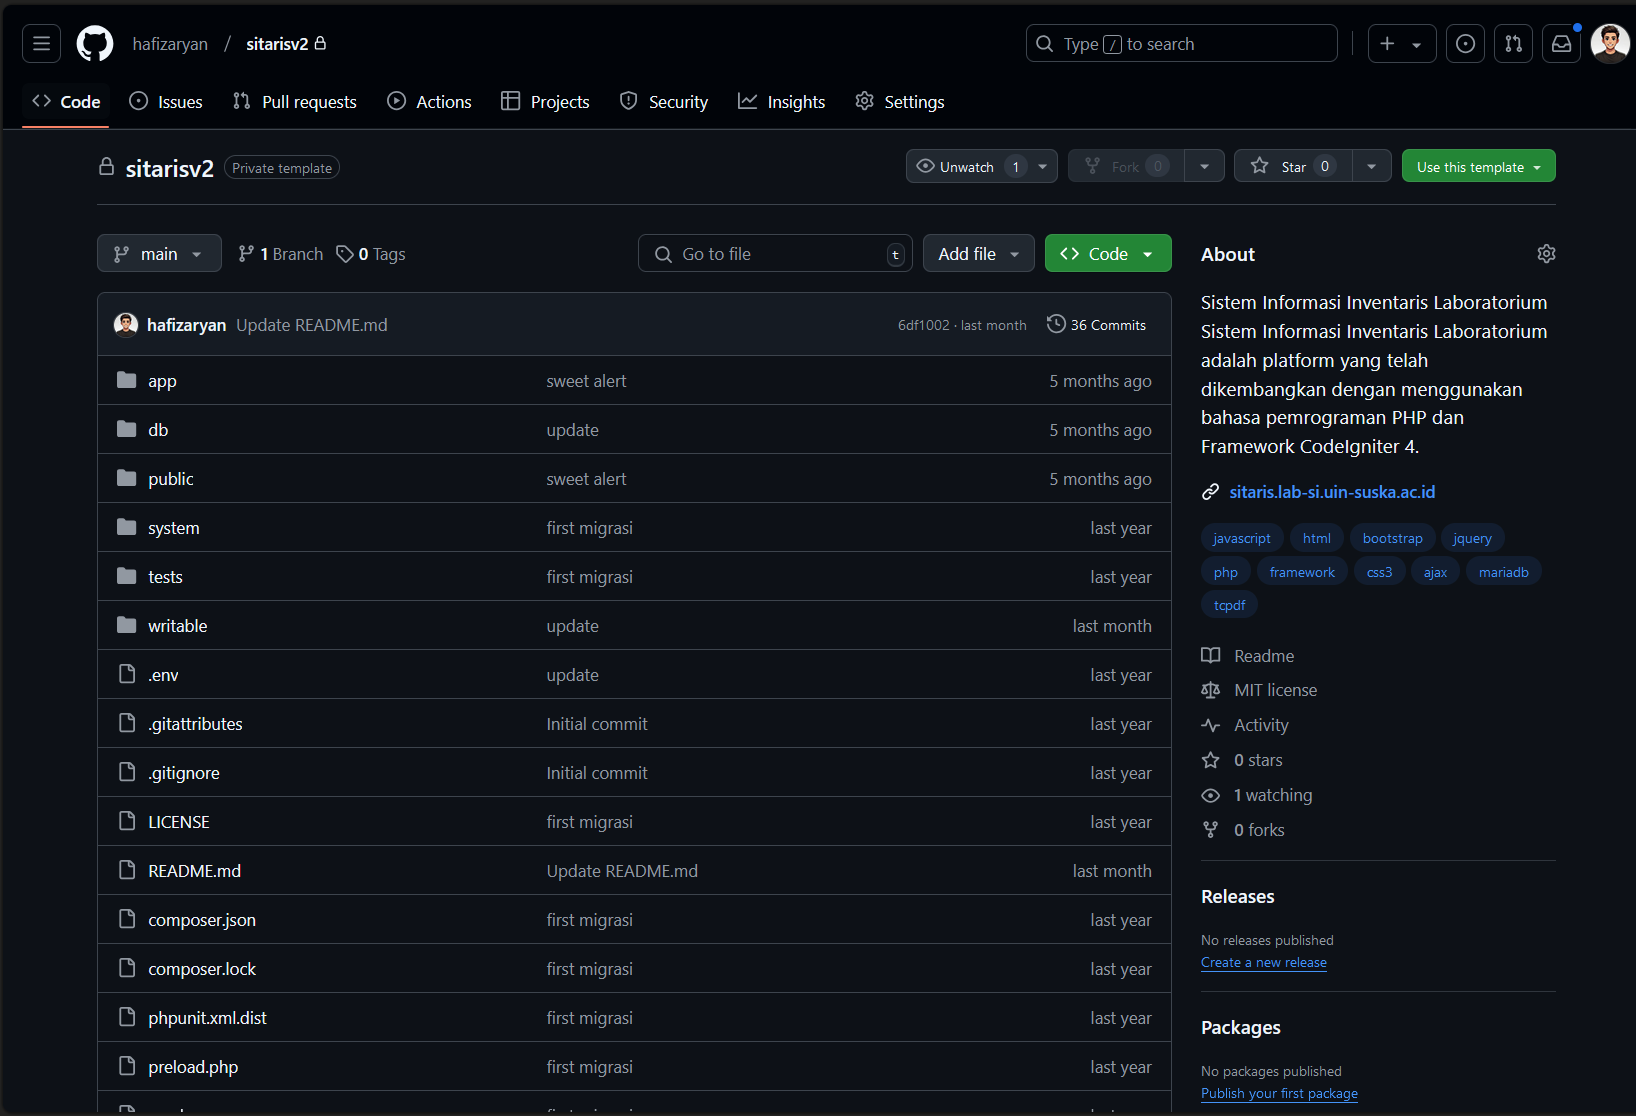
\includegraphics[width=0.82\linewidth]{konten/gambar/source-code.png}
	\caption{\textit{SOURCE CODE} SITARIS}
	\label{fig:source-code}
\end{figure}